% Created 2020-06-23 Tue 22:42
% Intended LaTeX compiler: xelatex
\documentclass{homework}
\usepackage{graphicx}
\usepackage{grffile}
\usepackage{longtable}
\usepackage{wrapfig}
\usepackage{rotating}
\usepackage[normalem]{ulem}
\usepackage{amsmath}
\usepackage{textcomp}
\usepackage{amssymb}
\usepackage{capt-of}
\usepackage{hyperref}
\usepackage{listings}
\class{CS 3141: Prof. Kamil's Algorithm Analysis}
\address{Bayt El-Hikmah}
\lstset{language=python}
\usepackage{lipsum}
\author{Musa Al`Khwarizmi}
\date{\today}
\title{Homework in Org-mode}
\hypersetup{
 pdfauthor={Musa Al`Khwarizmi},
 pdftitle={Homework in Org-mode},
 pdfkeywords={},
 pdfsubject={},
 pdfcreator={Emacs 26.3 (Org mode 9.3.7)}, 
 pdflang={English}}
\begin{document}

\maketitle
This is a demonstration of my homework \LaTeX{} class. It is an extension of the \texttt{amsart} and should have all of its functionality. These are some of the set symbols: \(\bC \supset \bR \supset \bQ \supset \bZ \supset \bN\), then some Greek and other mathematical symbols are, \(\al, \ep, \p, \ra, \Ra, \injective, \surjective, \bijective\). We can also insert multiple figures as seen in figure \ref{fig:org1c6c388}. There is also an \texttt{org-mode} version of this file\footnote{Tashfeen's \texttt{org-mode} configurations can be found \href{https://github.com/simurgh9/emacs786}{here}.}.

\begin{figure}[htbp]
\centering
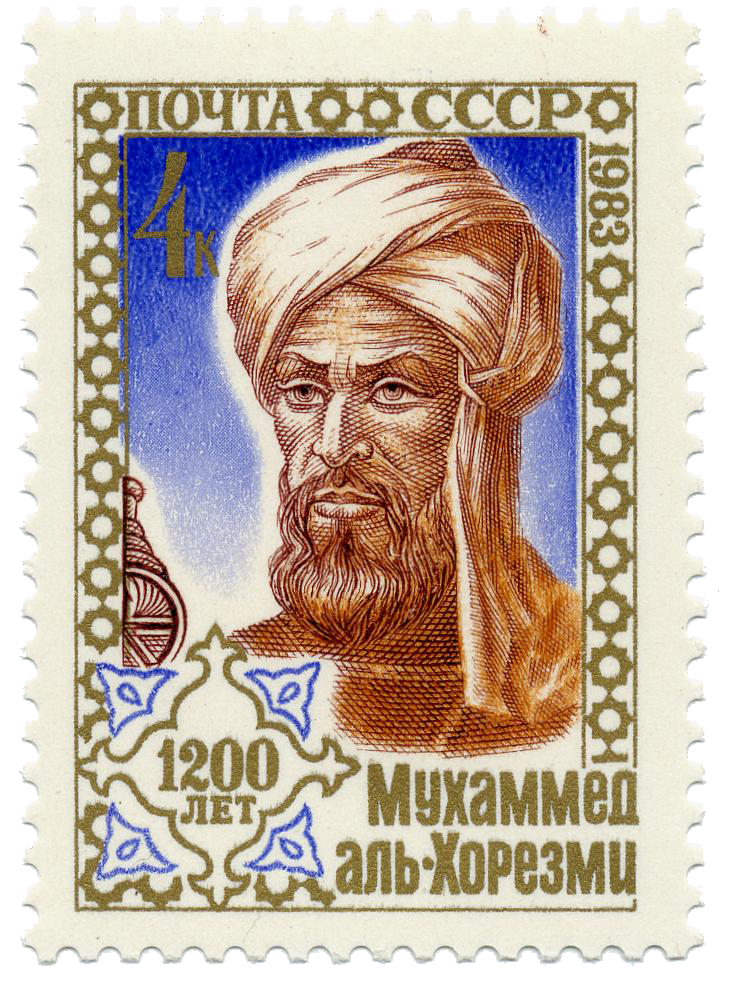
\includegraphics[width=0.3\textwidth]{../media/khwarizmi.png}
\caption{\label{fig:org1c6c388}Al`Khwarizmi}
\end{figure}

\begin{question}
Prove that \(\exists (x,y) \in \bZ\) such that \(x+y = 4\).

We show,
\begin{proof}[Proof of important theorem]
Four is the sum of two integers.

\(1,3 \in \bZ\) and \(1+3=4\).
\end{proof}
\end{question}

\begin{bonus}
Bonus Question Statement 

\lipsum[2]
\[
\zeta(x) = f(g(x)) \quad \text{ then according to the chain rule: } \quad
\derivative{\zeta} = \derivative[g]{f} \times \derivative{g}
\]
\end{bonus}


\begin{bonus}
Euclidean Algorithm

You may write code,
\lstinputlisting[language=Python]{../code/sample_code.py}
\end{bonus}

\begin{question}
What is the cardinality of Natural Numbers?

It is \(\aleph_0\) \cite{arlinghaus1996part}.
\end{question}

\begin{question}
Is the cardinality of Naturals and Reals the same because they are both infinite?

No, the cardinality of Reals is greater because they are also un-listable (uncountable).
\end{question}

\begin{question}[99]
Custom Numbering.

This question is numbered 99.
\end{question}

\begin{question}
Finally the numbered bullets are done with the \texttt{enumerate} package,

\begin{enumerate}
\item With just bullets,
\begin{itemize}
\item \textbf{Cats}
\item \emph{Dogs}
\end{itemize}
\end{enumerate}
\end{question}

\bibliographystyle{plain}
\bibliography{../test/citations}
\end{document}